%!TEX root = thesis.tex

\chapter{Information Based Perception}
\label{chapter:IBP}
The aim of this thesis is to create an agent based fire egress simulation that models human behavior as accurately as possible. Agent-Based Models (ABMs) consist of large-numbers of heterogeneous, autonomous entities inhabiting a spatially explicit, partially observable environment; macro level dynamics are said to emerge through the asynchronous interactions among these entities~\cite{Bonabeau:2002um,Epstein:1999vn}. Each of these individual entities will iterate through a sense-think-act cycle, where agents obtain information from their environment through {\em sensing}, make a decision through {\em thinking} and finally carry out their decision by {\em acting}. In many application areas in which ABMs have been applied, including crowd simulation, the emphasis is generally on describing thought processes accurately via rules. However, sensing is a critical aspect in the modeling process and can greatly impact both the individual and emergent properties of the system.

The terms perception and sensing are often used interchangeably in simulation literature. For clarity in explanation, the term {\em perception} is used to define the complete process of obtaining a set of (possibly filtered) \emph{percepts}~\cite{Russel:1995vi} from the environment. {\em Sensing}, on the other hand, is defined as the process of obtaining raw information from the environment; in this definition, and in this model, sensing is a part of perception.

As explained in the previous chapter, the proposed IBEVAC agent architecture is based on the central theme that humans are constantly processing information from the environment. The sense-think-act cycle used in agent based modeling is an excellent representation of the process by which humans get information from the environment, process this information and finally, act based on the decision made. Rather than what a human sees, hears or smells, what is more important is what he can mentally process. In fact, the entire human perception system can simply be considered to be an information processing entity. In this chapter the perception system of the IBEVAC agent based on this idea that perception is the process of gathering information from the environment is presented. This is called an \emph{Information Based Perception}(IBP) system.

Miller's seminal work~\cite{Miller:1956tr} on human cognition revealed two important characteristics of human cognition:
\begin{inparaenum}
\item Humans constantly group together similar data into \emph{chunks} of information.
\item At any given time, a human can only process a limited amount of information.
\end{inparaenum}
For IBP, the assumption is made that this limited capacity results in humans being attracted towards certain kinds of information, e.g.\ a bright light or a celebrity; this, in turn, results in other information in the environment being unnoticed. By organizing information into chunks, humans are able to use their limited information processing capability more efficiently. This ability can manifest itself in different ways. It can be reasonably assumed that during motion planning, humans will process a group of people coming towards them as a single obstacle rather than many individuals. This grouping not only helps the person make use of his limited information processing capacity more efficiently,  it also helps him/~her conform to social norms that instruct him/~her that walking through a group of interacting people would be rude.


This chapter explains and illustrates the working and usefulness of an Information Based Perception system for agents. It's viability is demonstrated through the implementation of a simple moving agent and by incorporating information based processing into the agent's navigation system. Why navigation only? Besides being one of the major components of Agent Based Crowd Simulation, navigation is also a process in which the effects of using a new perception system can be observed easily. The experiments towards the end of this chapter illustrate the significant effects that a modified sensing and perception system can have on an existing \emph{motion planning} algorithm.

The remainder of this chapter is organized as follows: Sect.~\ref{IBP:ReviewPerception} gives some background on how humans perceive the world around them; the IBP model itself is introduced in Sect.~\ref{IBP:Theory}; following this, Sect.~\ref{IBP:MotionPlanning} presents an analyses some of the existing work in motion planning; in Sect.~\ref{IBP:Results} presents the preliminary work done in visual and quantitative validation; finally, Sect.~\ref{IBP:Conclusion} concludes this chapter and gives an overview of the work that needs to be done.

\section{Limits of Human Perception}
\label{IBP:ReviewPerception}
In 1953, Hochberg and McAllister~\cite{Hochberg:1953eh} proposed their theory humans try to group together similar information so that information can be encoded in the simplest possible format. They call this \emph{the simplicity principle}. This idea was further extended by Miller~\cite{Miller:1956tr} originally proposed the idea that, at any given time, humans can only process a limited amount of information. He explained this as the human short term working memory having a limited capacity. Humans are aware of what is in their short term working memory and they arne't aware of what isn't stored in it. To enable humans to store more information in this limited storage space, humans ``chunk'' together similar information. He originally proposed that the short term working memory could hold $7\pm 2$ chunks. Recently, Cowan~\cite{Cowan:2001wi} has argued that this limit is actually $4\pm 1$ for most humans. Thus, even though a person's 5 senses are giving him a constant stream of information about the world, limitations of human short term working memory, force the person to act on the basis of only a fraction of this received information.

But then, which specific fraction of this received information is cognitively processed? Regarding visual perception, some studies~\cite{Itti:2001wa,OReagan:1999wj,Triesch:2003vz} have shown that humans only pay attention to certain salient features in the objects that they see. This results in them not noticing changes in items that are not of interest to them. O'Reagan et al.~\cite{OReagan:1999wj} classified elements as either central interest or marginal interest elements and prove that the internal representation of the visual world is rather sparse and essentially contains only central interest information and not information of objects of marginal interest. The world that we perceive around is a combination of this sparse visual world along with the information in our working short term memory received from our other senses.

Based on these studies, for our model, we make the reasonable assumption that the human brain uses some mechanism to determine the significance of a particular \emph{raw percept}. And the short term working memory stores the most significant information in its limited capacity. It is important to realize that this significance determination is done for \emph{all} information received, regardless of the source. We call this significance, the \emph{amount of information}.

The idea of considering the human perception system as an information processing system is not unprecedented. Broadbent~\cite{Broadbent:1965is} extensively discussed the idea of using information theory for modeling human perception. Various studies were presented that indicate that humans have an upper bound on their capacity for holding information for perception. For a single dimension, this limit is roughly estimated to be about 5-6 percepts. For more than one dimension, the number of discernible alternatives is larger but not as large as would be expected if each dimension was completely independent.

The idea of humans being able to process only a limited amount of information is not new to computer animation either. Hill~\cite{Hill:1999ww} was one of the first to introduce the importance of cognition in sensing. Courty~\cite{Courty:2003hy} used a saliency map based approach and Kim et al.~\cite{Kim:2005ub} used cost-benefit analysis in a decision theory based approach to determining the interest points. Grillon and Thallman~\cite{Grillon:2009hf}, this process of interest point determination was automated. They used criteria like proximity, relative speed, relative orientation and periphery to determine the interestingness of various features.

The majority of existing perception systems, consider perception to be only visual perception. Even in more detailed crowd simulation systems like LEGION~\cite{Still:2000tp} and MASSEgress~\cite{Pan:2006vp} perception is implemented to aid movement by detecting other obstacles and goals to enable planning a path towards the goal and to provide a collision free motion. The simplified IBP System implemented so far and demonstrated in this chapter is similarly limited, i.e.\ the IBP is modeled in the context of collision avoidance. The information which the agents perceive are dynamic obstacles, i.e.\ other agents or groups of agents. However, in the final IBEVAC agent the IBP will also observe events, cues and landmarks from the environment. These will, in turn, be used to learn more about the situation and environment and react appropriately to them.

In the present model, it is not proposed to model all the complexities of human perception and visual cognition, rather an agent based perception model for crowds is presented which can not only show a basic implementation of the idea of information based perception but can be easily extended when required, to model more complicated visual cognition. In order to demonstrate the effect of IBP on an agent's navigation system. It is first necessary to have an idea of existing navigation systems.

\section{Navigation Systems}
\label{IBP:MotionPlanning}

To recap, navigation is defined as the process or activity of accurately ascertaining one's position and planning and following a route. Thus we use the term \emph{navigation} to refer to the complete process of how a person moves from one point to another. Navigation itself can be broadly divided into 3 (or 4 parts) as shown in Fig.~\ref{fig:NavigationArchitecture} extracted from Fig.~\ref{fig:AgentArchitecture}. It was briefly explained in Sect.~\ref{IBEVAC:NavigationModule} and will be discussed in more detail in Sect.~\ref{CFW:NavigationModule}. In this section, \emph{motion planning} is discussed in more detail. It tries to ensure that the human does not go through another human being in the crowd.

\begin{figure}[!tb]
\centering
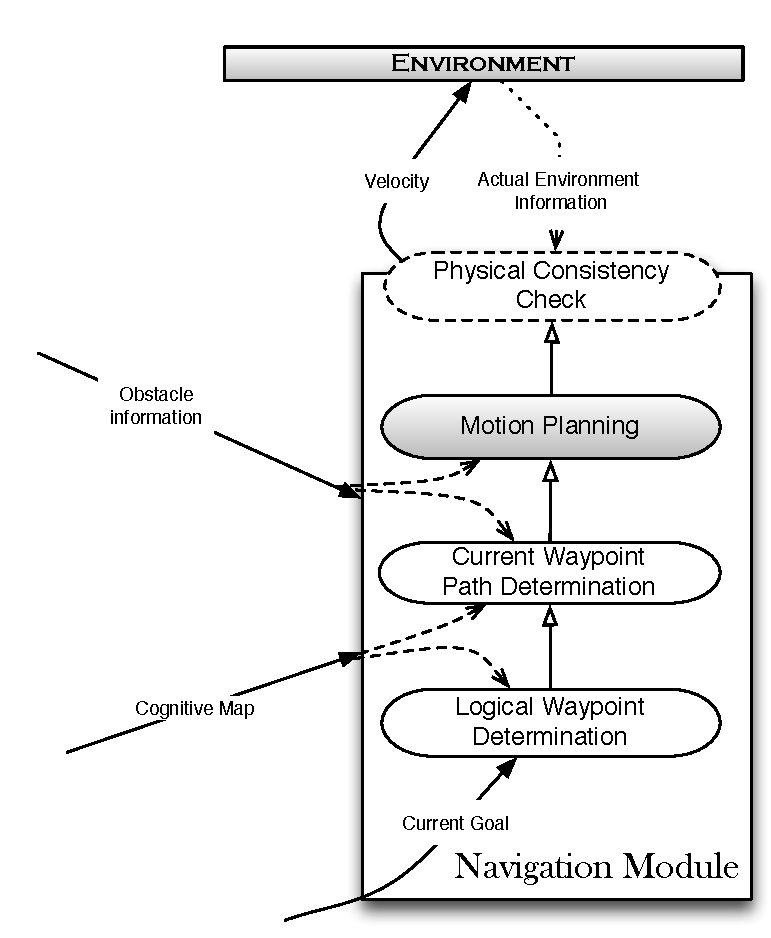
\includegraphics[height=4in]{fig-NavigationArchitecture}
\caption{Navigation Architecture}
\label{fig:NavigationArchitecture}
\end{figure}

There are various different approaches to motion planning. Klein and K\"oster~\cite{Klein:2009} uses an electric potential based model; positive charges are assigned to goals and negative charges to obstacles and agents. Okazaki and Matsushita~\cite{Okazaki:1993wh} use a similar approach of using magnetic poles instead of coulombic charges. In this section, only two of the most popular models for motion planning and collision avoidance used in agent based models, viz. the Social Forces model and the Reciprocal Velocity Obstacle (RVO) model are presented.

The social forces model was first introduced in Helbing's paper~\cite{Helbing:1995ie}. In this model, each agent is modeled as a particle that has multiple forces acting on it. Repulsive forces help in collision avoidance and attractive forces model goal directed and grouping behavior. Over the years, this model has been extended and combined with other higher level behavior models. For example, in~\cite{Kamphuis:2004uu} more complicated group movement was modeled with an underlying social forces model for collision avoidance. In his thesis, Still~\cite{Still:2000tp} criticized the heavily mathematical approach which, according to him, is too complicated to be the natural way in which humans try to avoid crowds.

Another ABM that is increasingly becoming popular for collision avoidance is based on the idea of using the relative motion of objects to determine their time to collision. A velocity is then selected which maximizes this time. This algorithm, based on RVO was first extended for use with multi agent systems in~\cite{vandenBerg:2008cq}. Since then there have been several modifications and improvements to the system but the underlying algorithm still remained the same. CLEARPATH~\cite{Guy:2009gu} which mathematically optimized RVO was the first to introduce a change in the underlying algorithm. Guy et al.~\cite{Guy:2010ko} introduced an entirely new approach to RVO that was based on computational geometry and linear programming. This method further improved the efficiency and smoothness of the system and was called \emph{RVO2}. In another article, Guy et al.~\cite{Guy:2010uv} introduced a personal space factor and an observation delay made the algorithm more appropriate for virtual humans.

Guy et al.~\cite{Guy:2010uv} introduced an extension to RVO in the form of a higher level navigation based on the principle of least effort. While it is obvious that rational humans would prefer taking the path of least effort, as was explained in Sect.~\ref{IBP:ReviewPerception}, humans do not have perfect knowledge or perfect calculation. Also, it is arguable whether humans are always rational enough to choose least effort as their goal.

There are a number of existing motion planning methods that can effectively and efficiently calculate trajectories that avoid all collisions for agents, even in relatively dense environments. For robots and computer games, this might be the ideal goal: perfect, smooth and efficient motion. However, for applications like simulation of emergency evacuation the goal is obtaining realistic motion and not smooth and efficient motion. While humans thrive to be mechanically efficient, this is hardly always the case. There exist, among other things, social norms and limits to mental processing capabilities that prevent individuals from following their ideal preferred path. Also, humans do not necessarily use optimality (in any sense) to determine their preferred path. The approach presented here is a more naturalistic one~\cite{Klein:2009} in that the author feels that motion planning models should explicitly consider and model human inadequacies and limitations.

In this chapter two additions to general motion planning algorithms are proposed:
\begin{inparaenum}
\item Group sensing for motion planning which results in agents avoiding clusters of other agents when choosing their collision free path.
\item Filtering of percepts based on the amount of information provided to model limited information processing capabilities of human beings.
\end{inparaenum}

Another important optimization that was introduced by Guy et al.~\cite{Guy:2010uv} was using the idea of clustering very distant objects into KD-trees to reduce computational cost. While this might sound similar to the idea that is suggested in this chapter, there are two fundamental reasons why this is different from the algorithm presented here: Firstly, the present model uses multiple levels of clustering which will be explained in more detail in Sect.~\ref{IBP:Clustering}. Secondly, the motivation and hence design is significantly different: clustering in IBP is used as a reflection of how agents perceive their environment and not an optimization for collision avoidance.

In the following section a method that will emulate how humans perceive groups whenever possible and a system in which the agents avoid these groups rather than individuals is proposed. This has been done using the Evolving Clustering Method (ECM)~\cite{Song:2001vg} and computational geometry based RVO2~\cite{Wilkie:2009da}. But our approach can, in principle, use almost any clustering and collision avoidance algorithms.


\section{The Information Based Perception Model}
\label{IBP:Theory}

\begin{figure}[!t]
\centering
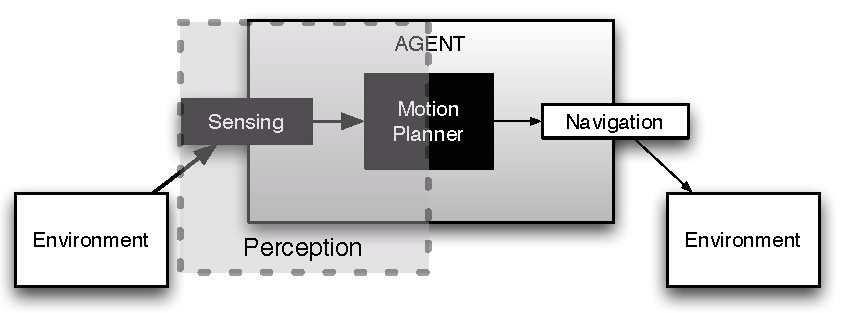
\includegraphics{PerceptionAndActing}
\caption[Perception and Acting]{An agent perceives and then acts}
\label{fig:AgentPerceptionAct}
\end{figure}

This section explains the Information Based Perception System. Figure~\ref{fig:AgentPerceptionAct} illustrates how motion planning works in an agent in terms of a sense-think-act cycle. An agent's perception can be described by a function $ f: Env \rightarrow p*$, where $p*$ is the set of percepts. Each percept $p$ is then processed by the agent in its decision making process, which in turn will determine an appropriate action for collision avoidance. In our case, the motion planning module is passed a set of percepts which consists of neighboring agents and static obstacles which it processes to find the most appropriate velocity for reaching the goal. Typically, this list of neighbors is a set of agents within some cone of vision or some distance away from the agent. In the proposed IBP, a modification to this traditional perception procedure is proposed such that it takes place in three phases: clustering, sensing and filtering. Figure~\ref{fig:AgentClusteredPerception} gives an overview of the process that is detailed in the following sections.


\subsection{Clustering}
\label{IBP:Clustering}
Central to our information based perception system is the definition of \emph{information units}. In traditional crowd simulation each individual agent or obstacle is considered as a percept, i.e. as an entity which should be processed by the motion planning system. The first assumption of our approach is that percepts can be both individuals and groups of other pedestrians. Whether an individual considers a group or individual is related to the {\em coherence} of the group and also the distance of the perceiving agent from the group. In order to achieve this, we perform a global clustering across the entire environment of agents. We create $n_l$ layers within the environment, each layer identifies and stores groups of a particular size, with increasing layer numbers storing groups of increasing size. The criteria which determines what actually constitutes a group is itself unknown and probably highly dependent on the individual. We make the assumption that only the proximity of the individuals to one another determine whether a collection of people is perceived as a {\em group}.

For reasons of efficiency we simplify things by performing a single clustering (for each level) for all agents at every time-step, the consequence is that we are implicitly assuming all agents have the same notion of what constitutes a group. In reality this assumption may be too strong, different people may have different criteria for what they perceive as groups.

While there are various clustering techniques that could be used for grouping agents, we chose to use ECM~\cite{Song:2001vg} because:
\begin{inparaenum}
\item It does not require the number of clusters to be predefined and
\item It can restrict the maximum radius of a cluster.
\end{inparaenum}
It is also important to remember that this clustering is done dynamically at \emph{each step} and not as a one time calculation of groups.


\begin{figure}[!t]
\centering
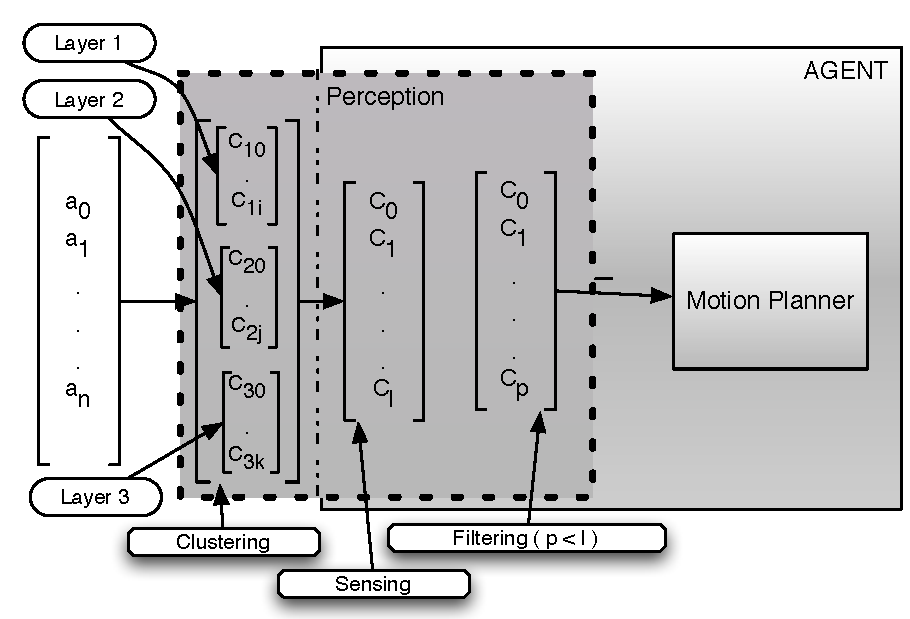
\includegraphics{ClusterProcessing}
\caption[Breakdown of the Perception Process]{Perception in agents takes place through three stages: (1)Clustering is done at a global level. The dotted line indicates this separation. (2) Sensing is the process by which the Agents perceive only a subset of this (3) Filtering further reduces the size of this list and models human visual cognition}
\label{fig:AgentClusteredPerception}
\end{figure}

First the number of clustering layers is decided. In Fig.~\ref{fig:ClusterLayer}, we illustrate information based perception using two layers. The algorithm starts by initializing a single agent as the first cluster, the maximum clustering radius for layer $i$, $r^{i}_{max}$ is fixed (\ref{firstLayerEq} and \ref{secondLayerEq}). Each subsequent agent is then compared with every existing cluster to assess its suitability for addition to that cluster. Suitability is determined by the distance of the agent from the cluster. If the agent lies within an existing cluster, it is simply added to that cluster without updating either the radius or the cluster center. Otherwise, the cluster whose center is closest to the agent is determined. If the agent can be added to this cluster, without exceeding the maximum allowed radius for the cluster, then the agent is added to the cluster and the cluster's radius, center and velocity are updated. On the other hand, if adding the agent violates the maximum radius criteria, then a new cluster is created at the location of the agent.

Once this process is completed for layer $i$, the process is repeated for layer $i+1$ until the clusters for all the layers are determined. This process is illustrated figuratively in Fig.~\ref{fig:AgentClusteredPerception}. The clustering function for layer $i$, $cf_{i}$ allocates one and only one cluster for each agent in each later. This can be represented mathematically as shown below:

\begin{equation}
   \forall a_{k} {\in} A \mbox{ }\exists j \in  [1 , m] \quad cf_{i} : a_{k} {\rightarrow} C_{ij} \mbox{ where } 1 {\leq} m {\leq} n
\end{equation}
\begin{equation}
  \\ \forall a_{j} \in A \quad C_{0j} = a_{j}
\end{equation}
\begin{equation}
 \\r^{1}_{max} = 2 \alpha * r_{a}
  \label{firstLayerEq}
\end{equation}
\begin{equation}
  \\ \forall i \geq 2 \quad   r^{i}_{max} = 2 \alpha * r ^{i-1} _{max}
   \label{secondLayerEq}
\end{equation}

Here $r_{a}$ is the average radius of an agent\footnote{In the experiments at the end of this chapter, it is assumed that all agents have the same radius. Hence, the radius of every agent is the same as the average radius.} in $A$ which is the set of all agents; $C_{ij}$ indicates cluster $j$ in layer $i$; $m$ is the number of clusters and $n$ is the number of agents. $\alpha$ is a parameter that determines the size of clusters and the range of each region (Fig.~\ref{fig:ClusterLayer}). Through experimentation we found the most pleasing results with $\alpha = 2$.

The ECM based clustering for each layer considers each agent exactly once so it the process has an asymptotic complexity of O($n^2$). At the end of each clustering, each agent belongs to a cluster. However, in the absence of nearby agents this might be a singleton cluster.

To correct certain undesirable behavior produced by ECM clustering, a modification was made to the algorithm. With large values of $r_{max}$, there is a chance that distant agents might be grouped into sparse clusters. To counter this problem, we define a \emph{checking circle} as a circle of radius $2 \alpha r_{a}$. If there are no agents within this checking circle, then the cluster is considered sparse and the cluster is removed. The sparseness check is done five times: First with the checking circle centered at the center of the cluster; and subsequently with the checking circles centered at a distance equal to half the distance from the center of the cluster along each of the coordinate axes.

\subsection{Sensing}
\label{IBP:Sensing}

Once the agents have been clustered, the next step is to make use of these clusters for motion planning. As previously explained, existing motion planning algorithms need a list of nearby agents and obstacles to determine the most appropriate velocity. The sensing module of our proposed perception mechanism uses the set of $n_l$ layers created in the clustering module. The list of things to avoid will now consist of agents, obstacles and groups of agents. This list of nearby objects is now calculated from the multiple clustering layers as shown in Fig.~\ref{fig:ClusterLayer}.

\begin{figure*}[!t]
\centering
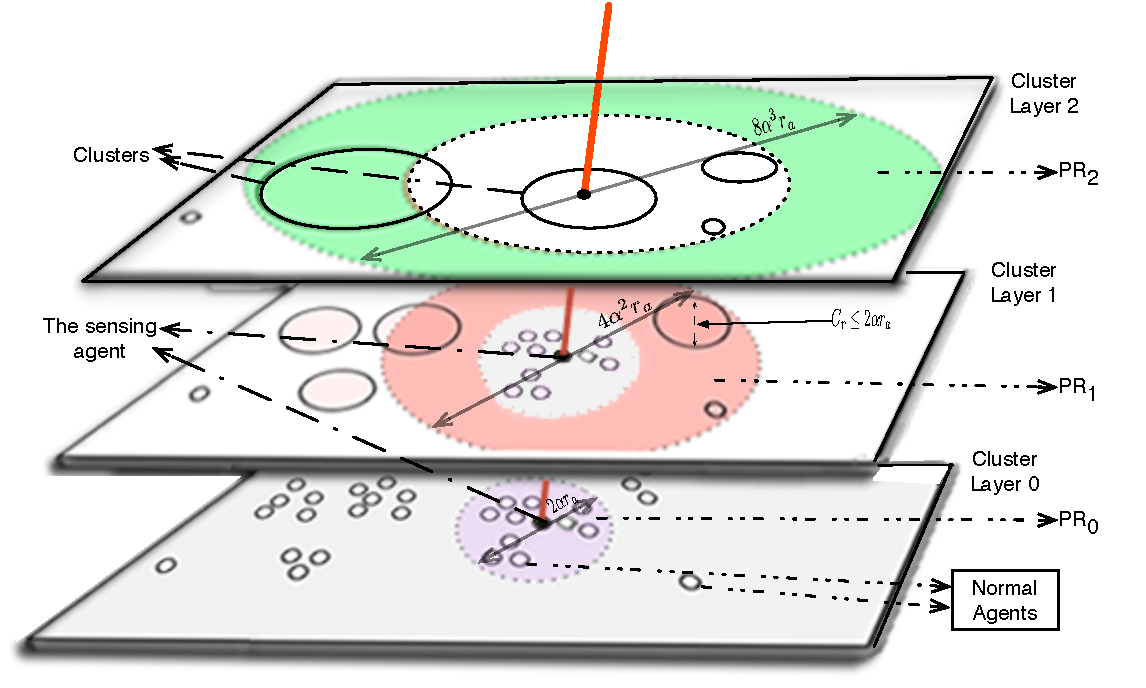
\includegraphics[width=\textwidth,height=3.5in]{AttemptedClusterLayer}
\caption[A Multi-layered Clustering Approach]{The figure illustrates how the opaque agent senses objects using 2 clustering layers. The bottom layer is the original environment and the two planes above show the two clustering layers. Clusters in layer 2 are generally bigger than in layer 1. Solid lined circles indicate the normal agents and the clustered agents. The dotted lines show the regions of perception. }
\label{fig:ClusterLayer}
\end{figure*}


From each cluster layer (explained in Sect.~\ref{IBP:Clustering}) a ring shaped {\em perception region} $pr_i$ is defined for each agent. This region can be considered as a modification of the sensor range which is used in most ABM.  In the first region ($pr_0$), immediately surrounding the agent performing the sensing, the agent perceives other individual agents from the clustering layer 0. This region extends to a distance $r_{pr_0} = 2\alpha *r_{a}$ from the agent's current location. For each subsequent region, the ring shaped region of sensing is from the boundary of the previous layer's region to the boundary of a circle of radius $2\alpha$ times the radius of the preceding region. So for region $pr_1$ the agent perceives groups of maximum size $r^{1}_{max}$, as long as the nearest edge of their minimum enclosing circle is within a distance $d$, such that $ r_{pr_0} < d \leq r_{pr_1}$. The result is a list of obstacles which consists of clusters of various sizes and individual agents.

\subsection{Filtering}
\label{IBP:Filtering}

As explained in Sect.~\ref{IBP:ReviewPerception}, a human being does not cognitively process every single object or obstacle that is within its vision. In other words, an agent can only process a limited amount of information and the information that is processed will be that which is deemed most interesting or important to the agent. So each object in the list obtained from perception is assigned an interestingness score of between 0 and 1 (1.5 for exceptional cases). During the sensing process each agent is given an information limit $a_{IL}$, indicating the total amount of information that can be processed by the agent. This limit is a parameter than can change as the stress level or other characteristics of the agent changes~\cite{Ozel:2001tn}.

For now, it is assumed that interestingness of an object depends on two criteria:
\begin{inparaenum}
\item The distance of the object from the agent.
\item The angle that the object currently forms with the direction of motion of the agent.
\end{inparaenum}
A third factor indicating the innate interestingness of the object being perceived can also be used. This can be used to represent a lot of other properties related to interestingness. For example, an object's speed, color, action or something more subjective, i.e.\ it is of interest only to this agent because of certain properties of the agent. For e.g., for a thirsty agent, a water cooler would be interesting whereas it is unlikely to catch the attention of someone else. A more exact definition of interestingness is not the focus of this report, but the general model here should be able to adapt to more sophisticated definitions. However, a notion of interestingness is required to extend IBP to detect events and cues in the situation and environment and this will be discussed in Sect.~\ref{IBP:Conclusion}.

Based on the two criteria, a score is given to each agent. A distance score of 1.5 is given if the distance between two agents is less than or equal to zero. This is to ensure that in high density scenarios where a collision does occur, a collision recovery mechanism is forced on the objects regardless of what angle or how interesting the object is. For other distances the following equation is used to calculate the score for a distance $d$. $\gamma$ and $k$ are parameters which were fixed at 5.0 and 1.11 respectively to get a curve as in Fig.~\ref{fig:DistanceScore}.
\begin{equation}
  	S_d = max(min(1.0, e^{\gamma / d} - k),0.1)
\end{equation}

\begin{figure}[!t]
\centering
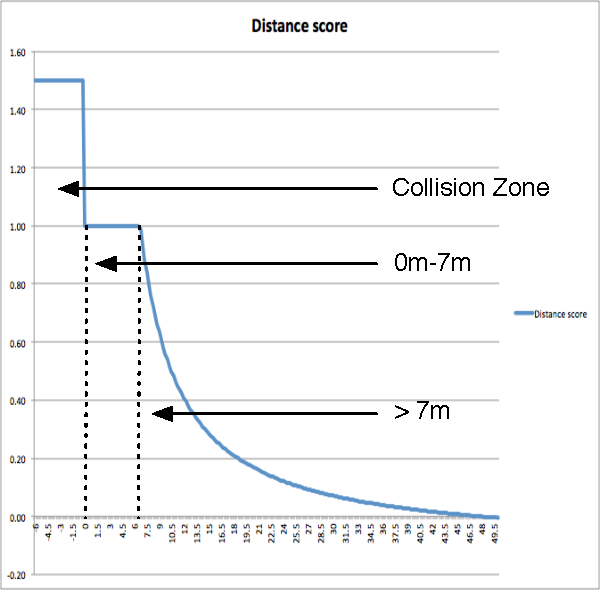
\includegraphics{distanceScore}
\caption[Distance Score]{This graph shows the variation of distance score with distance (in metres) used in experiments. A score of 1.5 if a collision has already occured, a score of 1 if it is within 7m and an exponentially decreasing score beyond that distance}
\label{fig:DistanceScore}
\end{figure}

An angle score of $1.0$ is given to all objects forming an angle of less than $a_{min}$ with the agent's direction. For all agents that form an angle of more than $a_{max} $ with the agent's direction,  a score of $ (1-\beta) $ is given. For our experiments a $\beta$ value of 0.9 was used and this is illustrated in Fig.~\ref{fig:AngleScore}. For all angles in between, the angle score linearly decreases to $ (1-\beta) $ from $1$. This is assigned based on the following equation (Fig.~\ref{fig:AngleScore}). All angles are in radians:
\begin{equation}
	S_{\theta} = 1.0 - (\beta * (a - a_{min} ) / (a_{max}-a_{min}))
\end{equation}

\begin{figure}[!t]
\centering
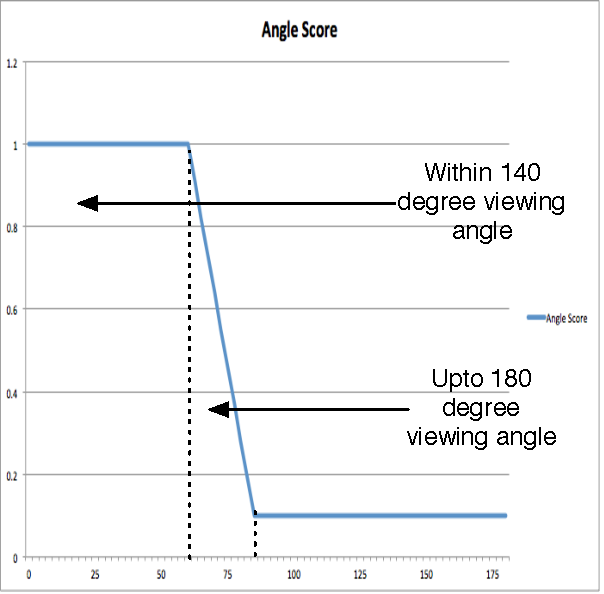
\includegraphics{angleScore}
\caption[Angle Score]{This graph shows the variation of angle score with the angle(in radians) formed by the object with the agent used in experiments. For objects forming an angle of less than $70^{\circ}$ (viewing angle $140^{\circ}$, a score of 1 is given. For objects forming an angle of up to $90^{\circ}$, the score linearly decreases to $0.1$ which is the angle score for all remaining obstacles.}
\label{fig:AngleScore}
\end{figure}

The final score for the object is calculated as the product of the $S_{\theta}$ and $S_d$~(as long as the distance score is not 1.5). This list of objects is then sorted on the basis of the score that is determined. Objects are then removed from the head of this list in turn and added to the final list of perceived objects as long as the cumulative score of all the perceived objects does not exceed the information limit for the agent, $a_{IL}$. All the remaining objects are dropped from the list of objects sensed and the final list of percepts $p*$ is obtained. In case two objects have the same score, the objects that are moving towards the perceiving agent are given precedence, subsequently closer objects are given preference.

This shortened neighbor list is passed to RVO2~\cite{Guy:2010ko} for calculating the velocity at each time step. Our hypothesis is that the 3-step perception process presented in this chapter provides an improvement in two ways: Firstly, there are fewer neighbors and hence, fewer constraints for a given sensor range. Secondly and more importantly, more human like results can be obtained as will be illustrated in Sect.~\ref{IBP:Results}.

\section{Results}
\label{IBP:Results}

Eventually, real world data, which would ideally be used for validation of the IBP model, will be collected. Nevertheless, this section presents a preliminary visual and quantitative validation of the IBP model. The ideas introduced in Sect.~\ref{IBP:Theory} are used as the basis for visually validating different aspects of the proposed model. For quantitative validation of the model, two measures are used: \emph{Effort Expended} and \emph{Inconvenience Cost}. In proposing their least effort based approach to motion planning~\cite{Guy:2010uv}, Guy et al. used a measure of effort expended to demonstrate the usefulness of their model. This effort was calculated as follows:

\begin{equation}
E = m \int \! (e_s + e_w |\vec{v}| ^2) \, \mathrm{d} t \quad \footnote{$e_{s} = 2.23 \frac{J} {Kg s}$ and $e_{w} = 1.26 \frac{Js} {Kg m^{2}}$ for an average human~\cite{Whittle:2006vsa}}
\end{equation}

In this section, the same measure of effort is used to analyze and validate the proposed IBP model. For simplicity, all agents are taken to have the same average mass of 70~kg.  However, this only measures the  mechanical effort involved. To measure the amount of effort spent in decision making, an \emph{inconvenience cost} measurement is introduced. The inconvenience cost is the number of time steps in which the agent chose a velocity other than its preferred velocity i.e., the number of times they had to avoid a collision.

Four different scenarios are considered to evaluate the overall performance. First, the effect that Group Based Perception can have on an agent moving through a crowd is demonstrated and the scenario is visually and quantitatively analyzed. Next, the effect of the multi-layered clustering on an agent moving towards a large group is similarly analyzed. Following this, the necessity of GBP in modeling the information processing limits of human beings is shown. Finally, the importance and relevance of the information threshold is demonstrated by demonstrating the effect that it can have on an agent.

\subsection{Group Based Perception}
\label{GBP}

\begin{figure}[!tb]
  \centering
   \subfloat[Traditional Circular Sensor Range]{\label{Exp1_RVO}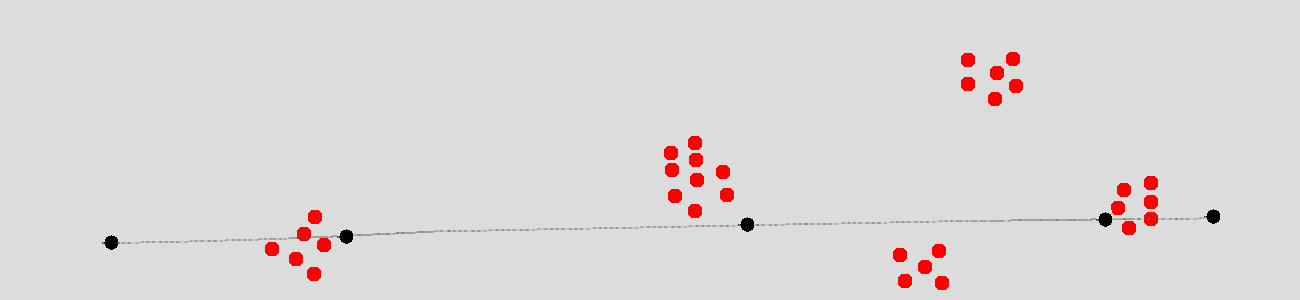
\includegraphics[width=\textwidth]{Exp1_RVO}}
  \\
   \subfloat[Group Based Perception]{\label{Exp1_GBP}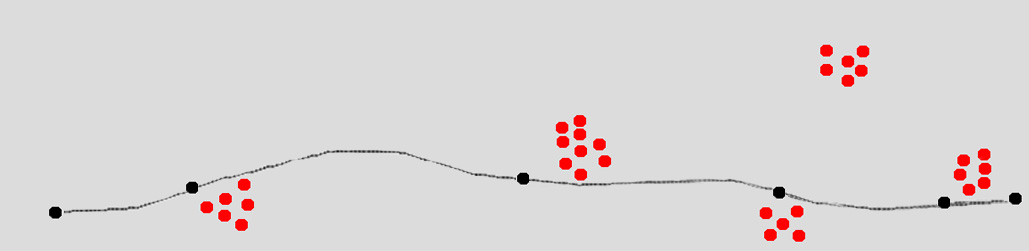
\includegraphics[width=\textwidth]{Exp1_GBP}}
   \caption{Experiment 1: Group Based Perception}
  \label{Exp1}
\end{figure}


In this experiment the results of using RVO2 with a traditional simple circular sensor range against RVO2 with a Group Based Perception system is shown. The intention is to show the effect of perceiving agents as groups. The hypothesis is that by perceiving groups as obstacles the simulation will generate more visually natural motion. In Fig.~\ref{Exp1}, there is a single black agent moving towards the right, and a number of groups of red agents moving towards the left. The black trail shows the path that is taken by the black agent. It can be seen that in Fig.~\ref{Exp1_RVO} where GBP was not used, the agent walked through other groups. Since RVO2 enforces each agent to do half the work to avoid collision, the agents within the group individually give way through its center for the oncoming agent to pass. At present this argument is based on the discussion in Sect.~\ref{IBP:ReviewPerception}, due to social norms and the human tendency to group information together people generally try to move around an entire group rather than walking directly through a group. As shown in Fig~\ref{Exp1_GBP} the GBP algorithm is capable of generating motion which avoids entire groups.

\begin{table}[tbp]
\caption{Quantitative analysis of Group Based Perception}
\begin{tabular}{>{\centering}p{1.2in}>{\centering}p{1in}>{\centering}p{1in}>{\centering}p{1in}>{\centering}p{1in}}
\tabularnewline
\hline\hline %inserts double horizontal lines
\multirow {2}{*}{Agent Considered} & \multicolumn{2}{c}{Effort ($ J{m}^{-1}* 10^5$)} & \multicolumn{2}{c}{Inconvenience Cost}\\
 & Without GBP & With GBP & Without GBP & With GBP
 \tabularnewline
\hline
Black Agent  & 71730 & 71726 & 120 & 148 \tabularnewline
All other agents (average) & 1884 & 1880 & 14.28 & 6.56 \\
\tabularnewline
\hline
\end{tabular}
\label{tab:Exp1_QuantitativeAnalysis}
\end{table}

An analysis of the effort expended and the inconvenience cost gives some interesting results. Since the simulation is executed for a given number of time steps, the effort expended is normalized with the progress towards the agent's goal. This is to avoid slow or stationary agents from being considered to be more efficient despite traveling a lesser distance. On comparing the normalized effort in the two scenarios of the black agent, it is found that despite having a much longer path, the GBP enabled agent expends slightly lesser (practically the same) amount of effort than the other. This is because the non-GBP agent has to slow down to wait for the other agents to give way before it can proceed and thus progresses less towards the goal.

The inconvenience cost comparison gives another interesting, though not surprising, result. The inconvenience cost to the black agent of using Group Based Perception is higher because of the more indirect path that it has to take. However, the average inconvenience caused to all the other agents is significantly lesser. This is consistent with the general human reluctance to inconvenience others. It also gives the interesting idea that even if the same amount of mechanical effort is expended in following two different paths, the amount of decision making required for each path might be significantly different.

\subsection{Effects of multi layered clustering}

\begin{figure}[!t]
  \centering
   \subfloat[Using traditional sensing]{\label{Exp2_RVO}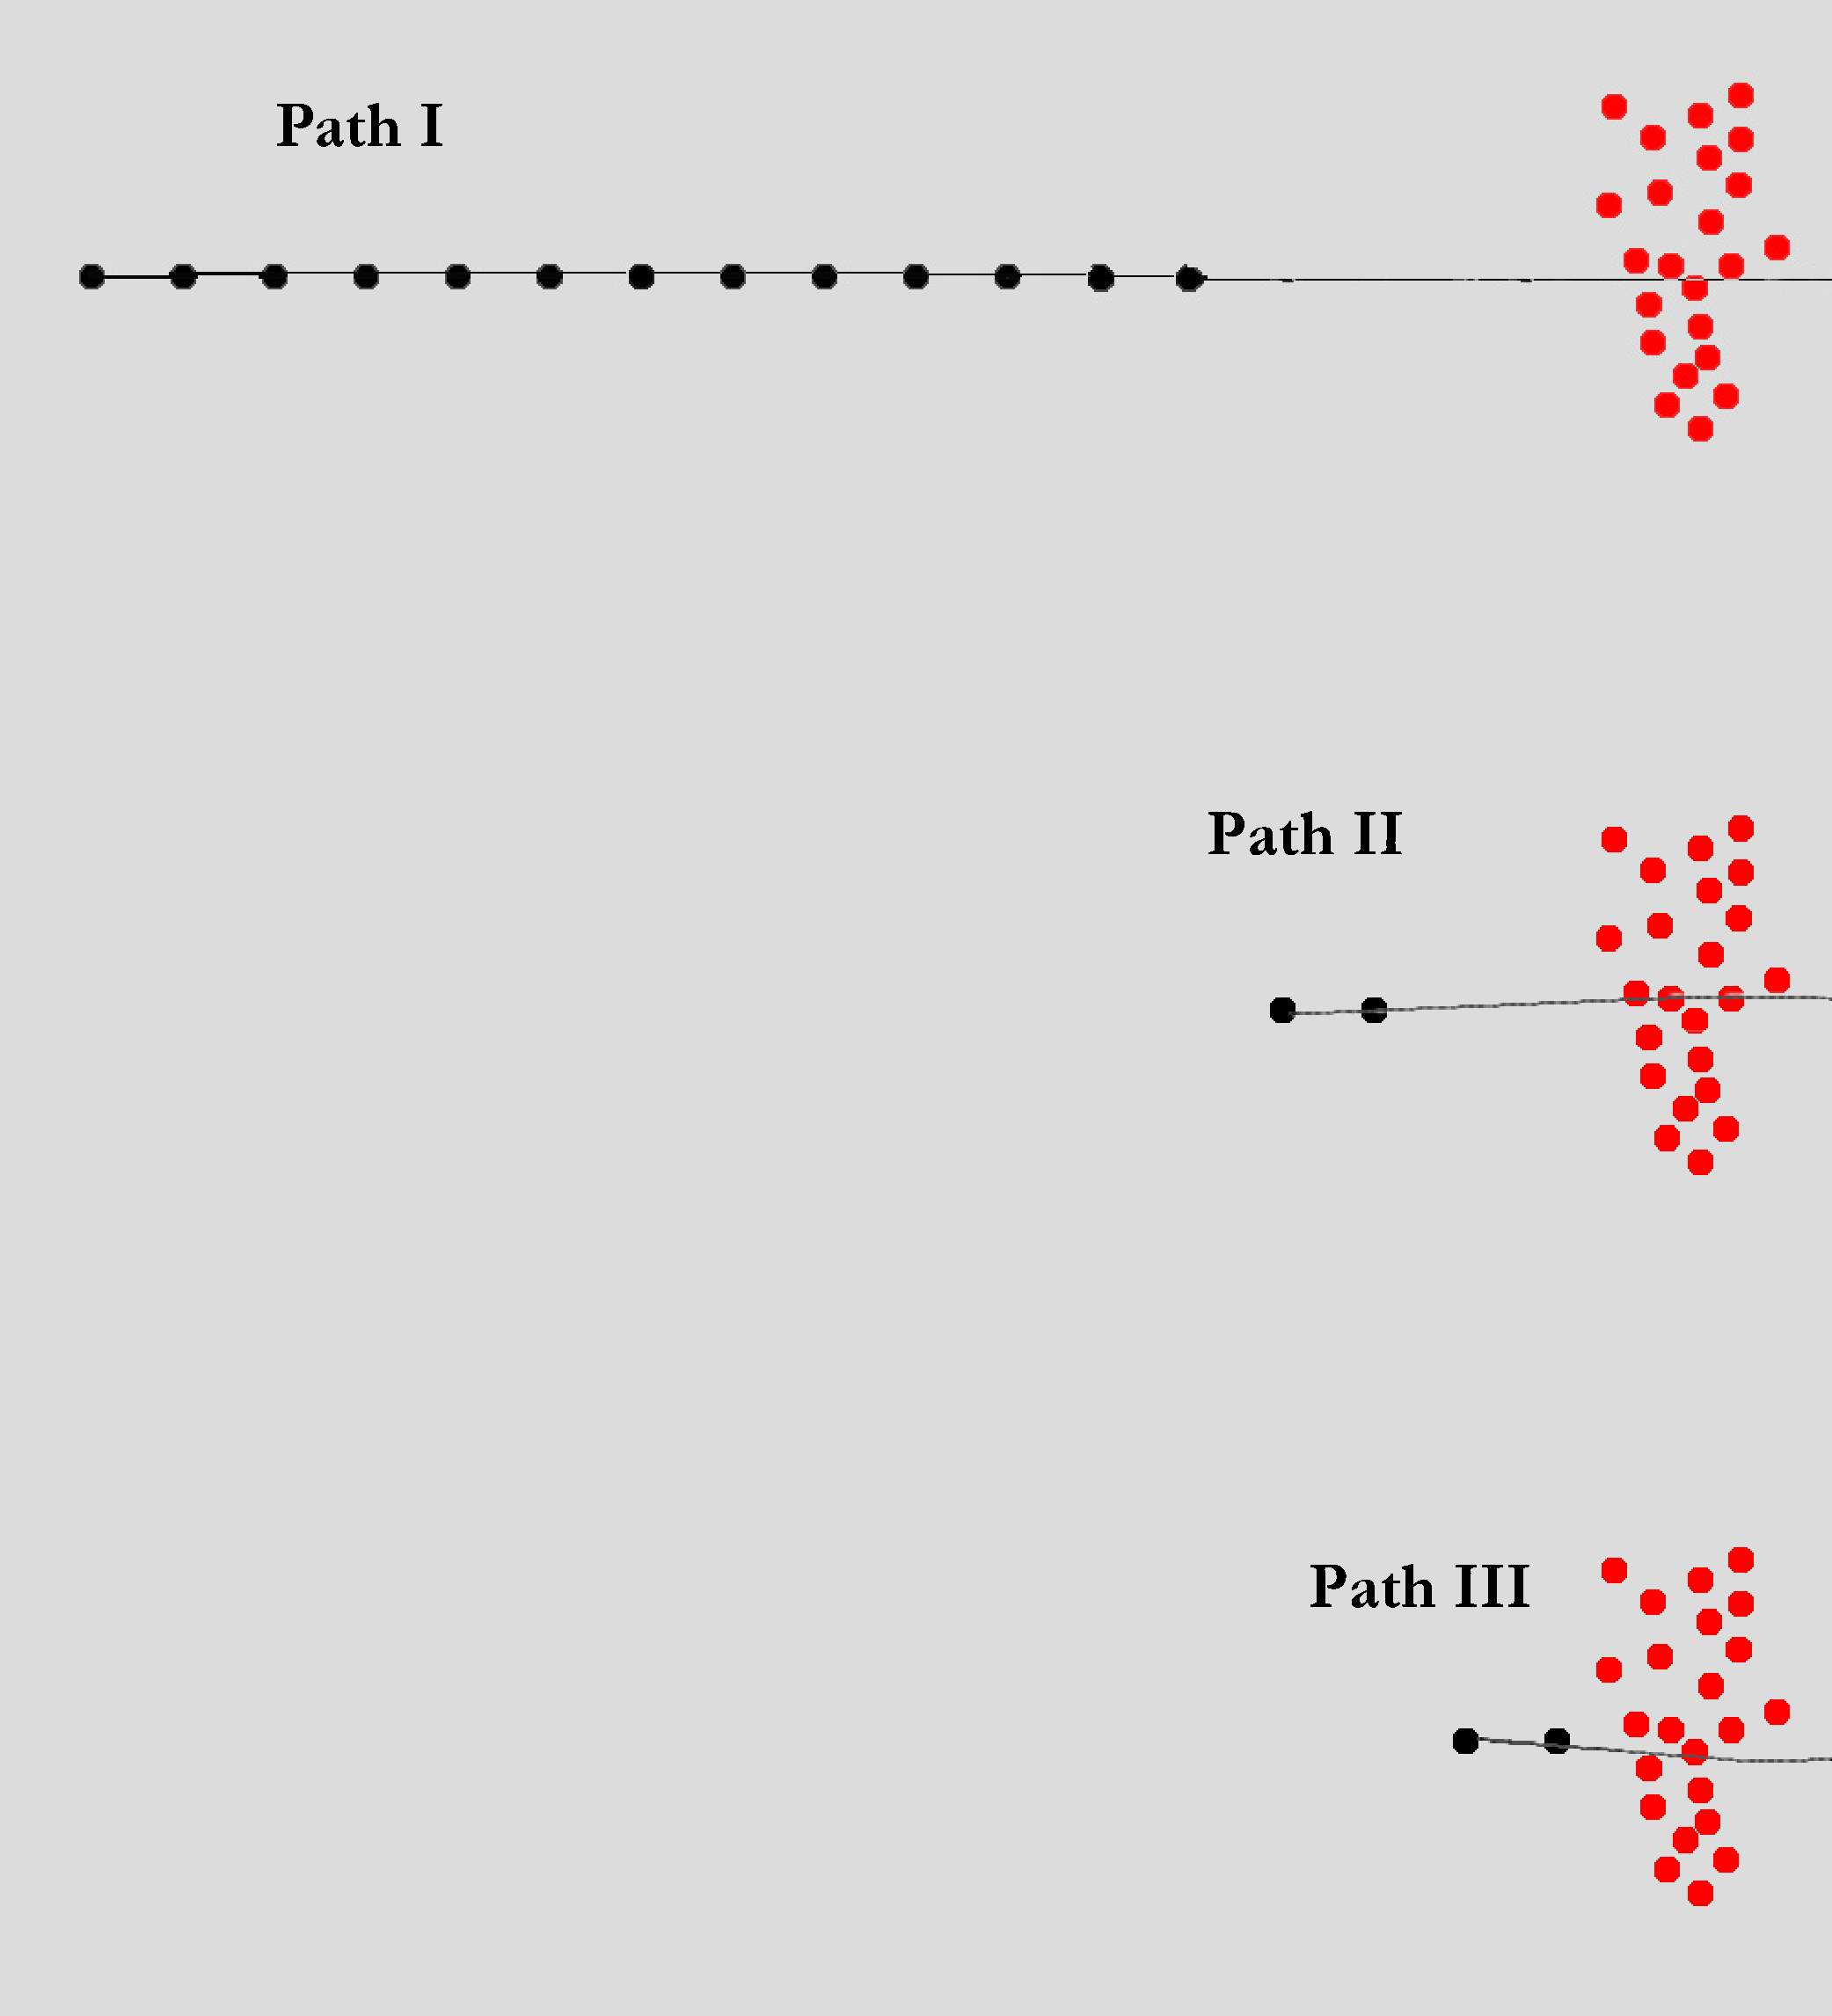
\includegraphics[width=7.5cm,height=12cm]{Exp2_RVO2}}
   \hspace{1pt}
  \subfloat[Using Group Based Perception]{\label{Exp2_GBP}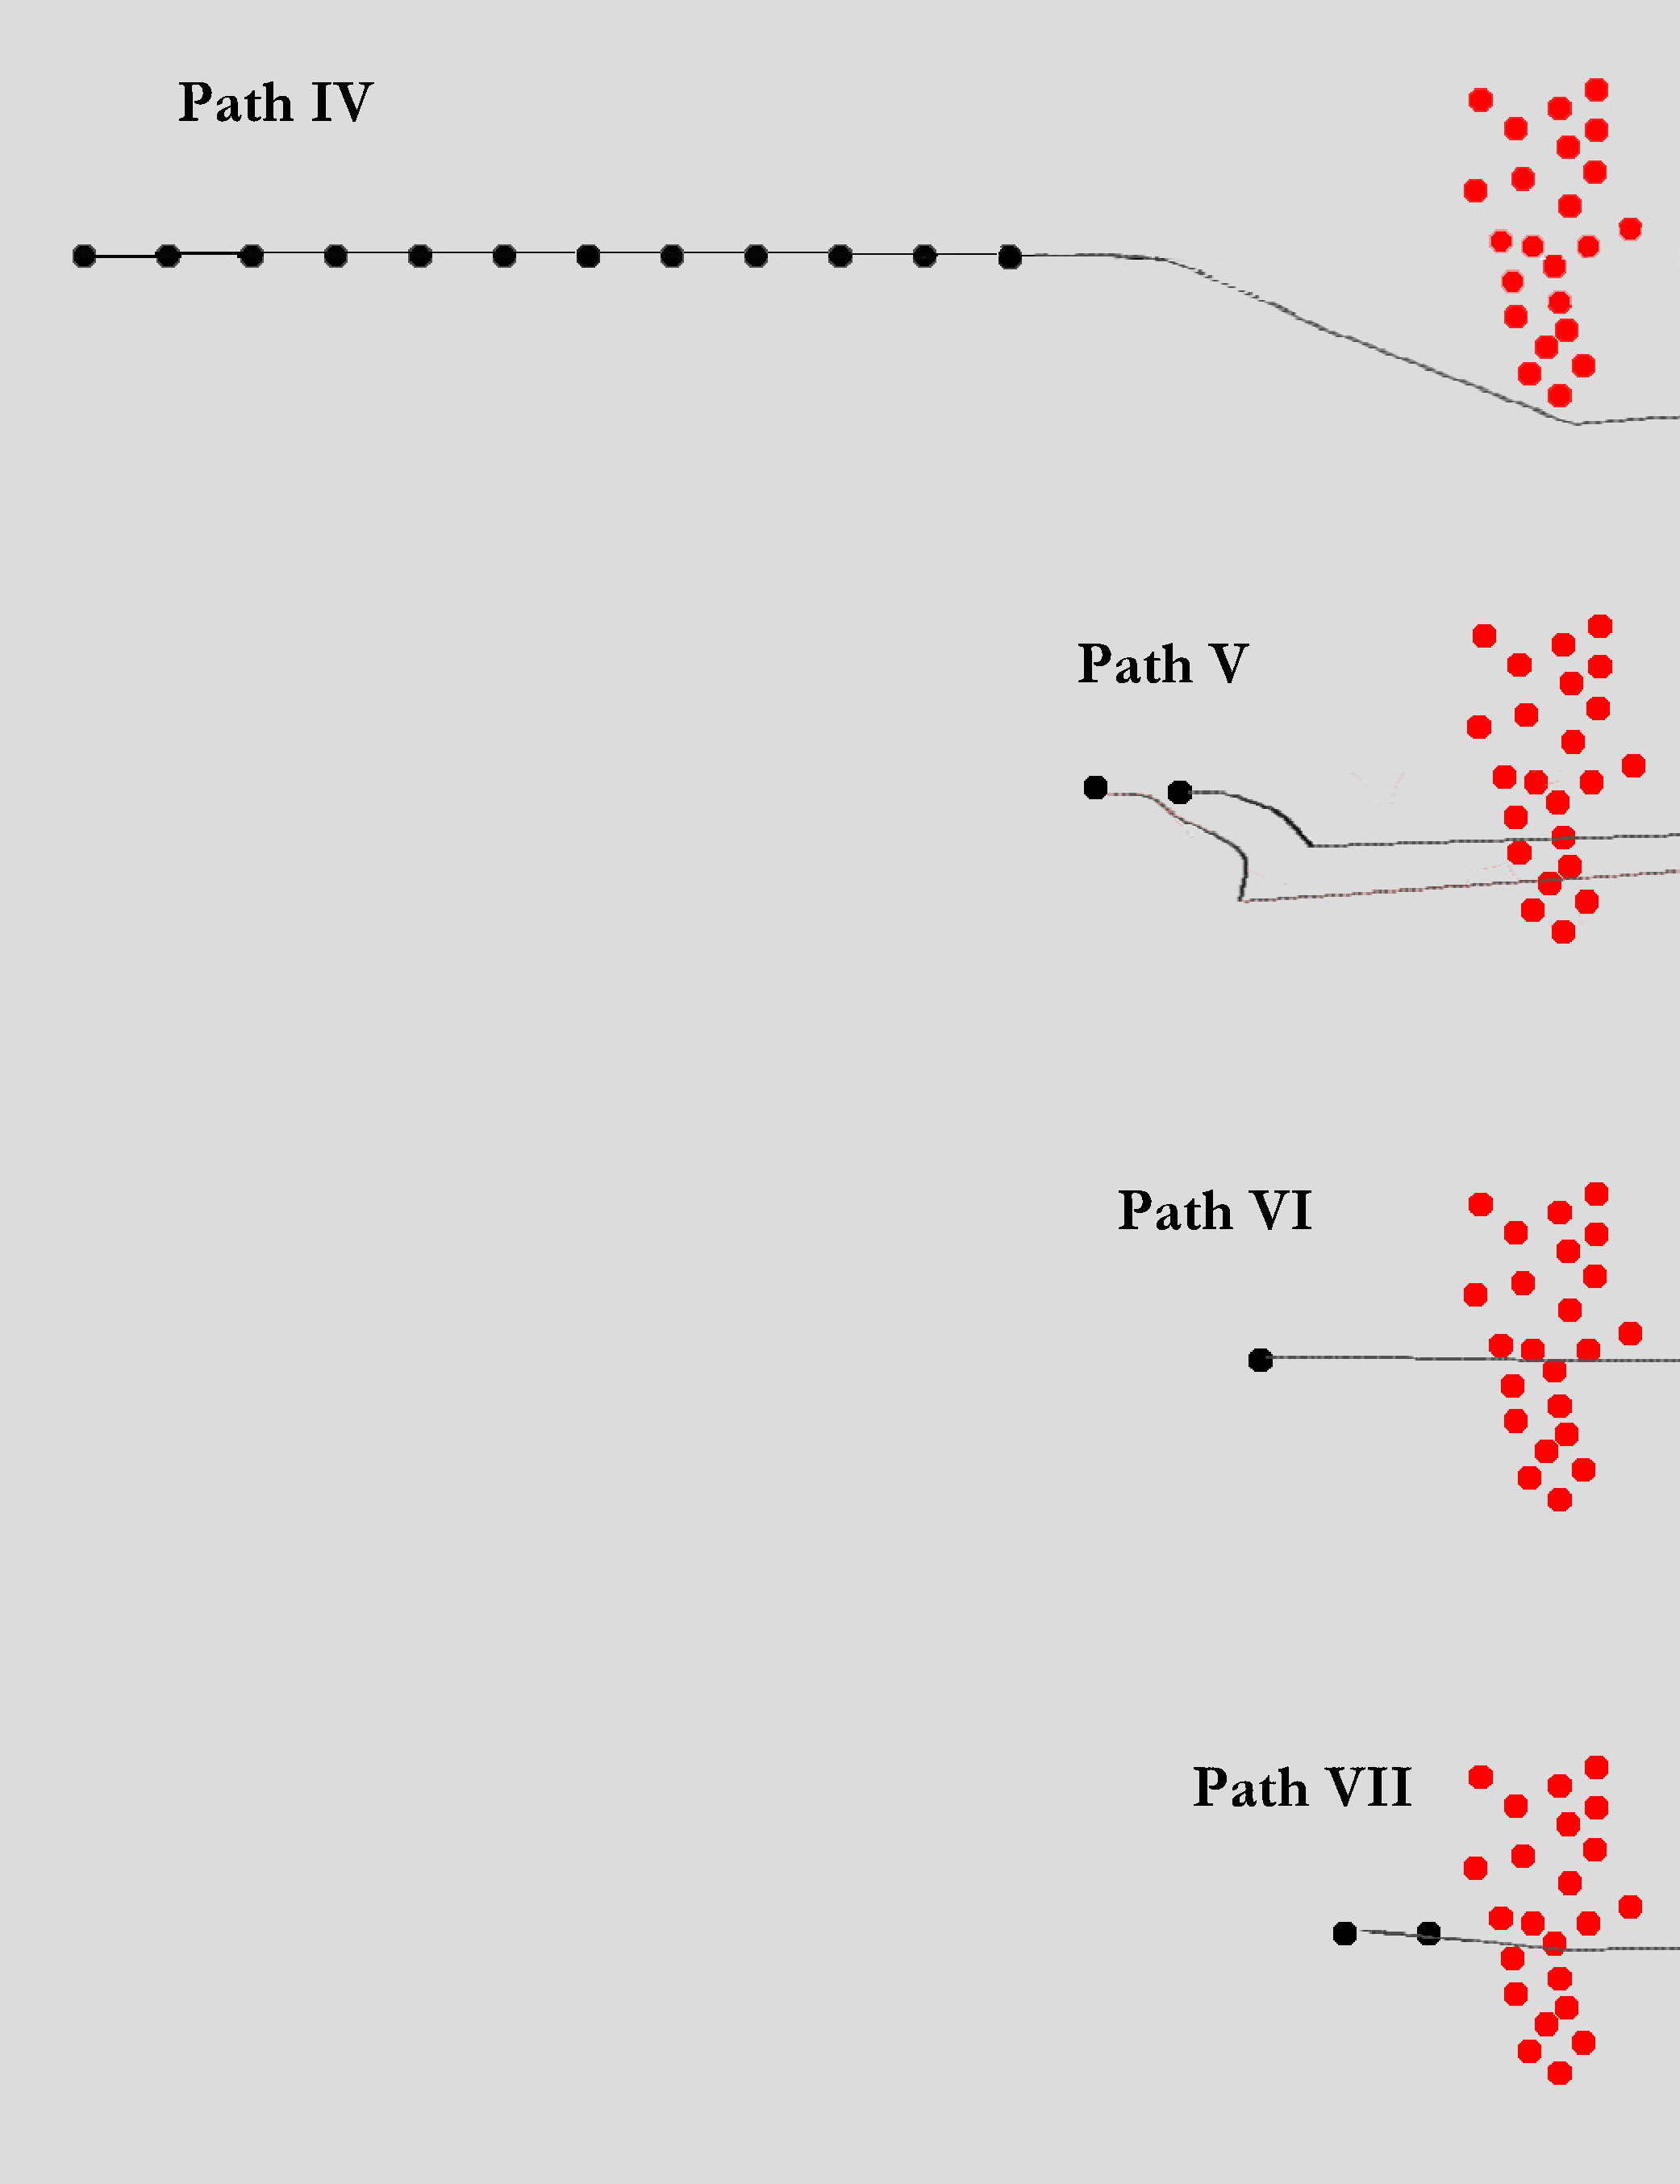
\includegraphics[width=7.5cm,height=12cm]{Exp2_GBP}}
  \caption{Experiment 2: Effect of multi layered clustering}
  \label{Exp2}
\end{figure}

In this experiment, the simple scenario where a single (black) agent had to get past a big group of agents to get to its goal is studied. The same experiment was performed by keeping the agent at different distances from the group. The objective of this experiment is two-fold. Firstly, it demonstrates the importance and the working of the multi-layered clustering (Sect.~\ref{IBP:Sensing}) used. Secondly, it demonstrates that when agents are very close to each other, where RVO2 already performs well, the Group Based Perception does not interfere with RVO2's functioning.

To recap, the multiple layers are used to describe groups of varying size at varying ranges of perception. This means agents will perceive other agents as groups or individuals depending on the distance; as an agent moves towards a group it will start to perceive the group as individual agents.

When GBP isn't used, the path followed does not change significantly with distance. The agents in the path of the black agent, give way to the agent, and the black agent just proceeds straight through the center of the large group (Path I in Fig.~\ref{Exp2_RVO}). In the last few cases (Paths II and III), the path is slightly different because the black agent does not have enough time to plan for a smooth, straight path and hence there is a slight deviation. Also, similar to the experiment in Sect.~\ref{GBP} it is forced to slow down in the process.

The result produced when GBP is used is more varied. Four distinctly different paths (labeled IV, V, VI and VII in Fig.~\ref{Exp2_GBP}) are produced based on how far the oncoming black agent is from the big group. At distances between 7-18m away from the center of the big cluster, the agent has enough time to perceive the group and avoid it completely (Path IV). At distances between 5-7m away, due to the size of the group, the agent gets too close to the group such that it then perceives the group as individuals. At this time (as described in Fig.~\ref{fig:ClusterLayer}) the agent performs motion planning on all the individual agents and as a consequence moves through the group, shown by path V. Path VI is obtained in a similar fashion; however, the black agent is too close to the group (4m away) to discern the effect of GBP. At distances closer than this (2-3m away), the path followed by the agent (Path VII) is exactly the same as that followed by the agent not using Group Based Perception (Path III). We argue that this type of flexibility in the perception of groups is critical to creating more natural behavior, humans will adapt what they perceive based on success or failure of their attempt to avoid larger groups.

\begin{figure}[!t]
  \centering
   \subfloat[Black Agent- Effort]{\label{Exp2_Black_Effort}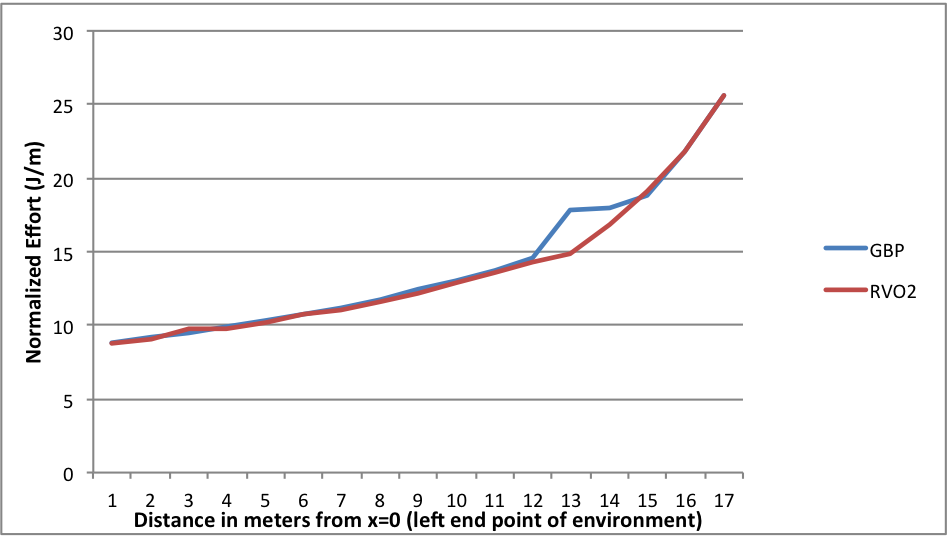
\includegraphics[width=7.5cm,height=5cm]{Exp2_Black_Effort}}
  \hspace{1pt}
    \subfloat[Black Agent- Inconvenience]{\label{Exp2_Black_Inconvenience}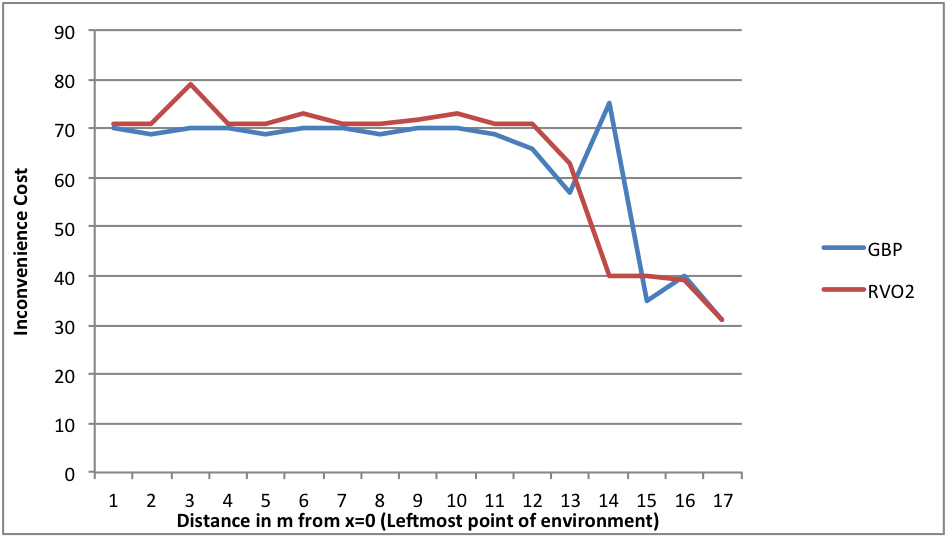
\includegraphics[width=7.5cm,height=5cm]{Exp2_Black_Inconvenience}}
  \\
  \subfloat[Remaining Agents- Effort]{\label{Exp2_Remaining_Effort}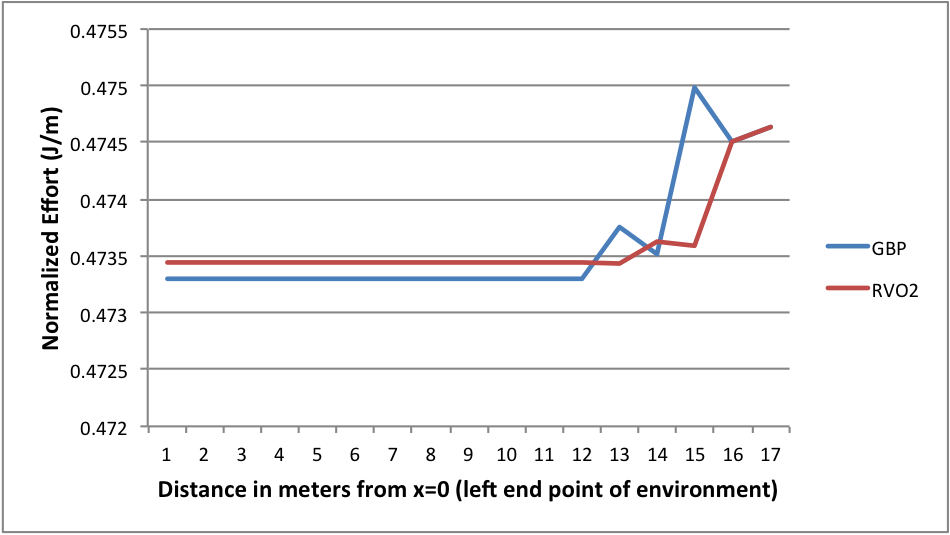
\includegraphics[width=7.5cm,height=5cm]{Exp2_Remaining_Effort}}
  \hspace{1pt}
  \subfloat[Remaining Agents- Inconvenience]{\label{Exp2_Remaining_Inconvenience}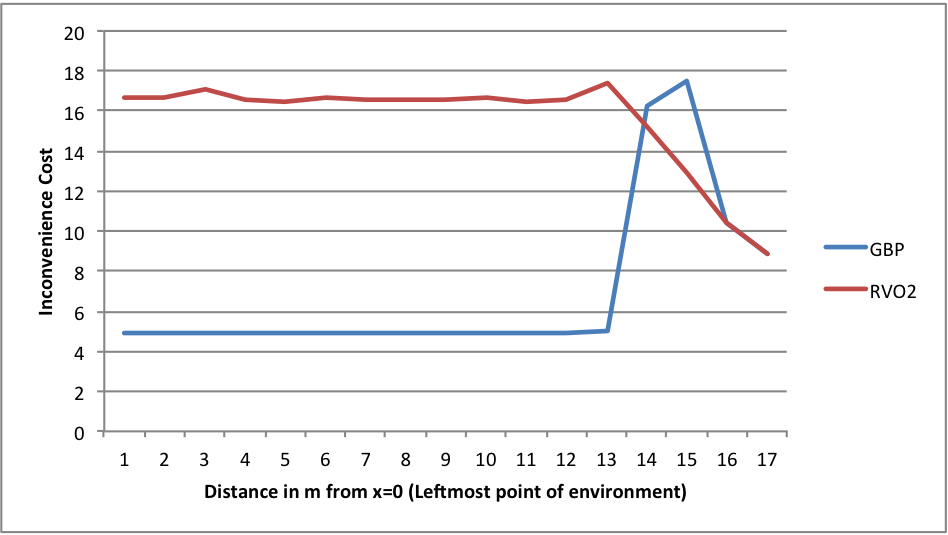
\includegraphics[width=7.5cm,height=5cm]{Exp2_Remaining_Inconvenience}}
  \caption{Experiment 2: Quantitative Analysis}
  \label{Exp2_QuantitativeAnalysis}
\end{figure}

Figures~\ref{Exp2_Black_Effort} and \ref{Exp2_Remaining_Effort} show a comparison of the effort expended by the black agent and the average effort expended by all the remaining agents while using a traditional sensor range and GBP. As in the previous experiment (Sect.~\ref{GBP}) there is hardly any difference in the effort expended in both scenarios (except for a slight increase for path V). However, an interesting pattern can be observed in the inconvenience measurement (Figures Figures~\ref{Exp2_Black_Inconvenience} and \ref{Exp2_Remaining_Inconvenience}). Firstly, the inconvenience for the rest of the group, is always lesser when GBP is used and almost the same for the black agent when path IV is followed. However, when path V or VI is followed there is a spike in the inconvenience curve. This can be explained by considering the fact that in both path V and VI, the black agent changes its planned path suddenly and decides to go through the group, thus not only increasing its own inconvenience but also the inconvenience caused to others in the group who have to move to give way to the agent. Finally, when path VII is followed both the effort and inconvenience count are exactly the same as for path III.

\subsection{Filtering necessitates Group Based Perception}


\begin{figure}[!t]
  \centering
  \subfloat[Initial Scenario]{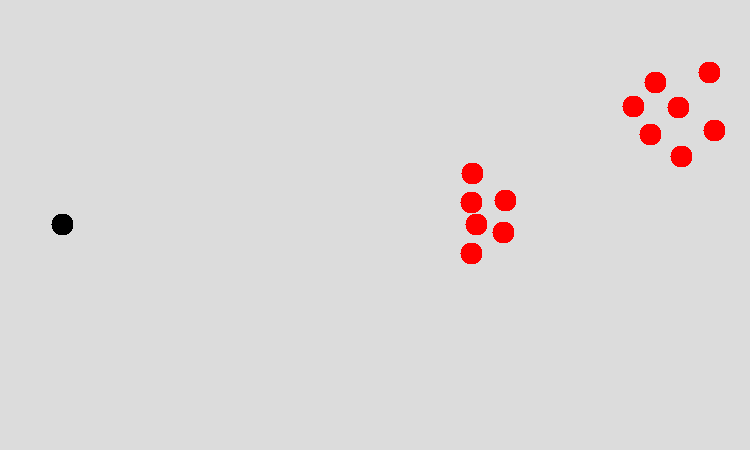
\includegraphics[height=5cm]{Exp3_initial}}
   \\
    \subfloat[Info limit of 4, without GBP]{\label{Exp3_4_RVO}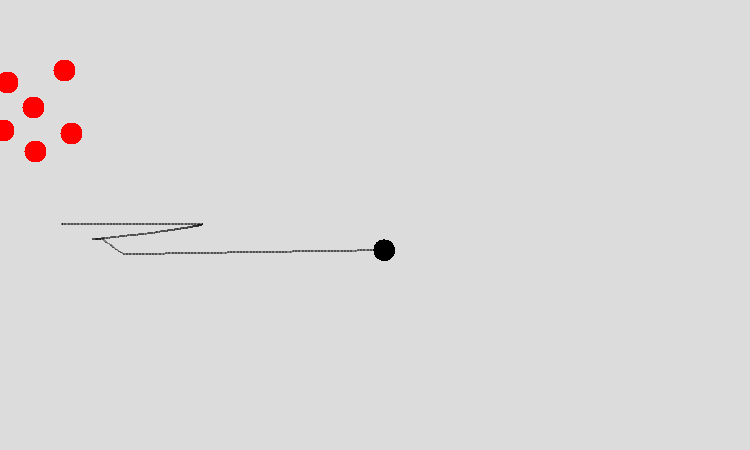
\includegraphics[width=7.5cm,height=4cm]{Exp3_4_RVO}}
    \hspace{1pt}
   \subfloat[Complete knowledge, without GBP]{\label{Exp3_full_RVO}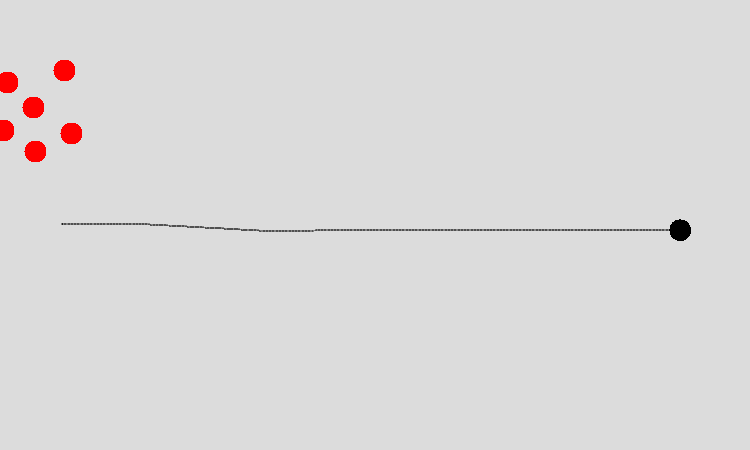
\includegraphics[width=7.5cm,height=4cm]{Exp3_full_RVO}}
  \\
  \subfloat[Info limit of 1, with GBP]{\label{Exp3_1_GBP}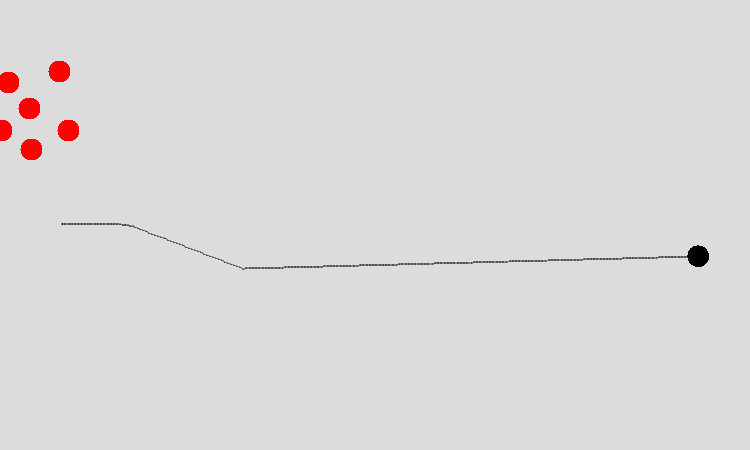
\includegraphics[width=7.5cm,height=4cm]{Exp3_1_GBP}}
  \hspace{1pt}
  \subfloat[Info limit of 4, with GBP]{\label{Exp3_4_GBP}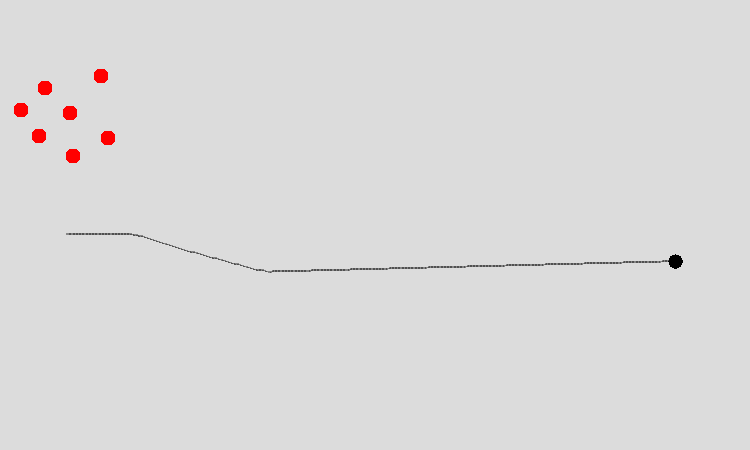
\includegraphics[width=7.5cm,height=4cm]{Exp3_4_GBP}}
  \caption{Experiment 3: The necessity of Group Based Perception}
  \label{Exp3}
\end{figure}

In Sects.~\ref{IBP:Theory}, the fact that humans have limited information processing capacity was explained. In this experiment, it is demonstrated that if a human being's limited information processing capability is to be modeled, it is necessary to use Group Based Perception. This is done by observing the simple scenario of an agent moving towards two groups of other agents (Fig.~\ref{Exp3}). When no information limit is imposed on the agent, and a normal circular sensor range is used, the agent, as expected, follows a nice straight path through the center of the group. However, when an information limit of $a_{IL} = 4$ is imposed on the agent, the black agent, does not perceive all the individual agents in the group and  as a result it is forced to reconsider its path mid-route. As a result, the irregular trail shown in Fig.~\ref{Exp3_4_RVO} is obtained. However, in the same situation, when Group Based Perception is used, the agent smoothly avoids the whole group (Fig.~\ref{Exp3_4_GBP}). In fact, this smooth path is obtained for as low a limit as $a_{IL} = 1$ (Fig.~\ref{Exp3_1_GBP}).

\subsection{Effect of filtering of percept information}

\begin{figure}[!tb]
  \centering
   \subfloat[Initial Scenario]{
\includegraphics[height=5cm]{Exp4_initial}}
   \\
   \subfloat[InfoLimit 3: Step 1]{\label{Exp4_3_1}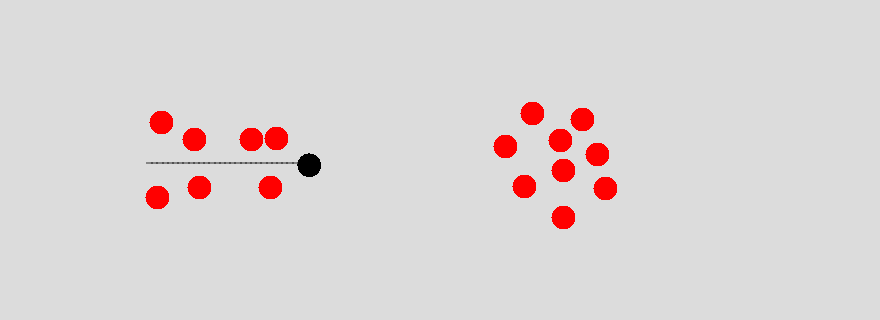
\includegraphics[width=7.5cm,height=4cm]{Exp4_3_1}}
  \hspace{1pt}
    \subfloat[InfoLimit 5: Step 1]{\label{Exp4_5_1}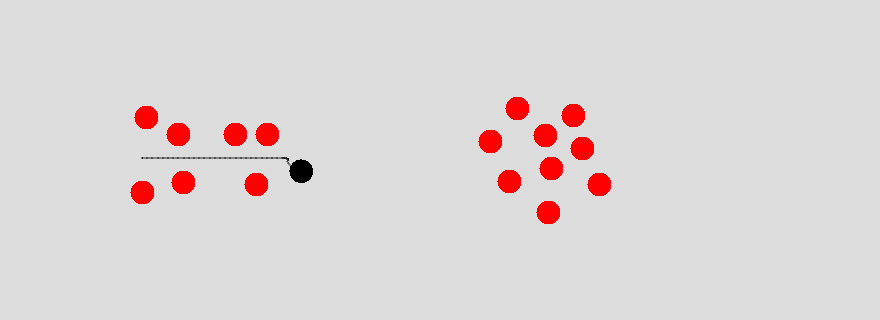
\includegraphics[width=7.5cm,height=4cm]{Exp4_5_1}}
  \\
  \subfloat[InfoLimit 3: Step 2]{\label{Exp4_3_2}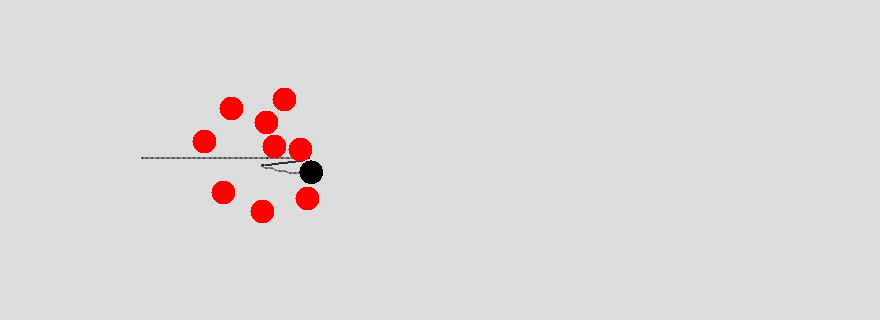
\includegraphics[width=7.5cm,height=4cm]{Exp4_3_2}}
  \hspace{1pt}
  \subfloat[InfoLimit 5: Step 2]{\label{Exp4_5_2}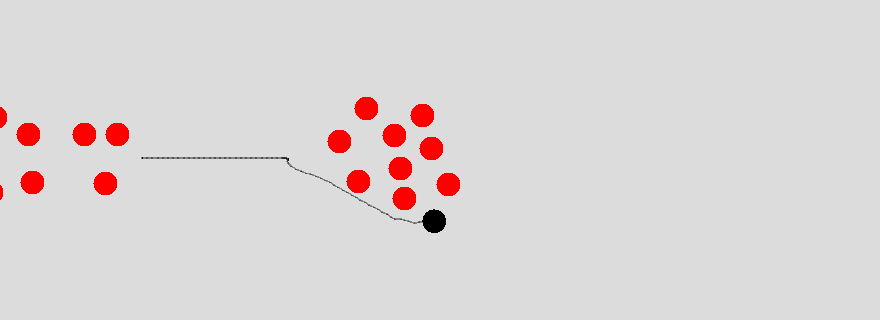
\includegraphics[width=7.5cm,height=4cm]{Exp4_5_2}}
  \caption{Experiment 4: Effect of filtering of percept information}
  \label{Exp4}
\end{figure}

The final experiment (Fig.~\ref{Exp4}) demonstrates the effect of filtering, i.e.\ having limits on the information processing capabilities of the agents. The scenario consists of an agent moving towards a collection of individuals (moving towards the agent) followed by a group of agents behind the set of individuals. In the first case an information limit of $a_{IL} = 5$ is set so that the agent is continually capable of perceiving a larger number of other agents and groups. In the second scenario a lower limit of $a_{IL} = 3$ is used such that the agent isn't initially capable of perceiving the group behind the individuals. Figure~\ref{Exp4_5_1} shows how agents perceive the cluster that is farther away, even when there is an immediate collision to avoid. Figure~\ref{Exp4_5_2} shows that the agent manages to move around this group because it had a head start in planning - i.e.\ , it considered the group early when avoiding collisions. In the second scenario it could process a maximum of 3 or 4 percepts at any given time because of the lower information limit. Due to this, as seen in Fig.~\ref{Exp4_3_1}, the agent cannot see beyond the immediate obstacles in front and does not prepare in advance to avoid the larger group. Once the agent finally perceives this group, it is too late to move around this group as it perceives the group as individuals and then moves through the group as in Fig~\ref{Exp4_3_2}.

This experiment illustrates how small differences in the information limit can generate different forms of behavior in the agents. Interestingly, the info limit of 3 and 5 correspond to Cowan's finding~\cite{Cowan:2001wi} that all humans can cognitively process only 3-5 chunks of information at any given time. Clearly the value of the limit is critical to behavior, it is also proposed that this limit will change with personal characteristics and the emotional state of the agents. In fact this varying limit of perception may be an important factor for collisions in actual crowds, this is especially relevant in emergency egress scenarios where stress and collisions are critically important to safety planning. We plan to attempt to quantify this information limit through experimentation in future work.

\section{Summary and Future Work}
\label{IBP:Conclusion}
In this chapter, the Information Based Perception model for agents which is based on perceived information rather than spatial distance has been introduced. The argument that this is a more appropriate model of human perception for crowd and egress simulation has been made. The behavior of this system has been illustrated through experiments. It has been shown and argued that this creates more realistic group avoidance behavior. The idea that humans have limited perception capacity such that they only process certain obstacles more relevant to collision avoidance is incorporated; this in turn will result in a reduction in efficiency of collision avoidance.

As mentioned earlier, for the IBEVAC model, the IBP model will have to be extended so that during filtering it can recognize cues that contain event and environment information and pass it to the appropriate modules for processing. Also, critical to the model is the quantification of information limits and appropriate definitions of interest; real world experiments will be conducted to attempt to quantify these parameters. The third criteria which was mentioned in Sect.~\ref{IBP:Filtering}, i.e.\ the inherent interestingness of the object, will also be the subject of these real world experiments. In emergency situations, according to Ozel~\cite{Ozel:2001tn}, humans start perceiving cues in the environment differently. This idea was touched upon in the literature review chapter. The idea of modeling different cues and their effect on the agent's information processing capabilities as suggested by Kuligowski~\cite{Kuligowski:2009un} is an idea that will be discussed in more detail in Chapter~\ref{chapter:ConclusionAndFutureWork}. As mentioned by Hill~\cite{Hill:1999ww} there is also a reciprocal effect of cognition on perception where agents would turn towards objects of more interest. It is planned that this will also be incorporated into later version of the IBP model. The next chapter concludes this report by giving a brief description of the other parts in the model that have been considered so far and a more complete description of how the final IBEVAC model will look.


